%!TEX root = thesis.tex
\chapter{Infinite Projected Entangled Simplex State}
\label{chapter:ipess}
\section{Simplex-solid State}
\label{solidstate}
The simplex-solid state of an SU(N) quantum anti-ferromagnet was derived by Arovas \cite{} and the most significant conclusion is that any simplex states could be described by a natural generalization of the AKLT \cite{} valence bond solid state which means that the bond signlets of the AKLT could be extended to N-site simplices.

The concept of simplex-solid states ansatz were introduce by Xie et al \cite{}. The tensor-network representation of simplex states is called projected entangled simplex state (PESS) which is also considered as an extension of PEPS \cite{} obeying the area law of entanglement entropy and characterizing any states if the dimension of the virtual bonds are large enough. The difference from the PEPS is that the entanglement among the virtual particles is described by entangled simplex tensors which depend on the structure of PESS. For example, in Fig. \ref{fig411}(b) there are three virtual particles within the simplex state, so the entangled simplex tensor $S_{mnl}$ is a rank-3 tensor.

\begin{figure}[ht]
	\centering
	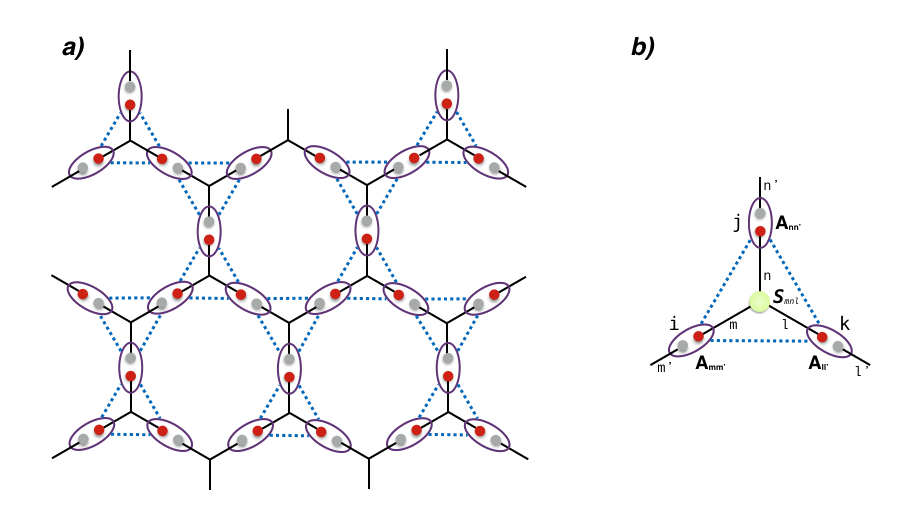
\includegraphics[width=0.80\textwidth]{figures/fig411.png}
	\caption[The picture of the main idea of itebd.]{The red and blue tensor denotes on \textit{odd} and \textit{even} sites. The yellow one are time evolution operators $e^{-\tau H_{k,k+1}}$, $e^{-\tau H_{k+1,k}}$}
	\label{fig411}
\end{figure}

For illustrating how to write down the formulation of the PESS wave function, we begin from a simple system, the spin-2 simplex state on an infinite Kagome lattice \cite{}. See Fig. \ref{fig411}(a) each physical $S=2$ states on the lattices could be treated as a symmetric superposition of two virtual $S=1$ spins. According to the theory of AKLT, each neighbor simplices (triangles) share a single site symmetrically which also means that the $S=1$ spins could be assigned to one of the simplices (vertex-sharing). Hence, there are three $S=1$ spins in each simplex states. From the features of the $SU(2)$ group, the decomposition of the direct-product of three integer spins is written as, 
\begin{align}
	\label{su2}
	n \otimes n \otimes n = [a_0 \times 0] \oplus \dots \oplus [a_k \times k] \oplus \dots \oplus [a_{3n} \times 3n] \\
	a_k = \begin{cases}
		2k + 1 & \text{, $k \leq n$} \\
		3n + 1 - k & \text{, $k > n$} 
	\end{cases}
	\quad \text{, } k = 0, 1, \dots , 3n ,
\end{align}
where $a_k$ is a constant and $k$ express the $k$th irreducible representation. Now that we can write down the product of the spins in the simplex as,  
\begin{align}
	\label{111}
	\barbelow{1} \otimes \barbelow{1} \otimes \barbelow{1} = \barbelow{0} \oplus \left( 3 \times \barbelow{1} \right) \oplus \left( 2 \times \barbelow{2} \right) \oplus \barbelow{3},
\end{align}
and show that there is an unique spin-singlet state. The result encourage us to define a virtual singlet on simplex,
\begin{align}
	\Ket{\psi_{\alpha}} = \frac{1}{\sqrt{6}} \sum_{\left\{ s_i s_j s_k\right\}}{S^{\alpha}_{s_i s_j s_k}\Ket{s_i, s_j, s_k}},
\end{align}
where $s_i,s_j,s_k$ are $S=1$ virtual spins located at site $i,j$ and $k$ containing in the simplex $\alpha$ and $S^{\alpha}_{s_i s_j s_k}$ is the Levi-Civita antisymmetric tensor $\varepsilon_{ijk}$ [Fig. \ref{fig411}(b)]. For mapping the two virtual $S=1$ spins to the spin-2 subspace, we defined the projection operator $P_i$ on each site,
\begin{align}
	P = \sum_{s_i,s^{\prime}_{i}}\sum_{\sigma_i}{A^{\sigma_i}_{s_i,s_i^{\prime}}\Ket{\sigma_i}\Bra{s_i,s_i^{\prime}}}
\end{align}
where $\Ket{\sigma_i}$ is a basis of the $S=2$ spin at site $i$. $A^{\sigma_i}_{s_i,s_i^{\prime}}$ is a projected matrix whose components are filled by the Clebsch-Gordan coefficients,
\[
	\begin{aligned}
		&A_{11}^2 = A_{33}^{-2} = 1, \\
		&A_{12}^1 = A_{21}^{1} = A_{23}^{-1} = A_{32}^{-1} = \frac{1}{\sqrt{2}}, \\
		&A_{13}^0 = A_{31}^{0} = \frac{1}{\sqrt{6}}, \\
		&A_{22}^0 = \frac{2}{\sqrt{6}},
	\end{aligned}
\]
Now that we can write down the wave function of the simplex-solid state,
\begin{align}
	\Ket{\Phi} &= \bigoplus_i P_i \prod_{\alpha}{\Ket{\psi_{\alpha}}} \\
	&= \Tr \left( \dots S_{s_i s_j s_k}^{\alpha} A^{\sigma_i}_{s_i,s_i^{\prime}} A^{\sigma_j}_{s_j,s_j^{\prime}} A^{\sigma_k}_{s_k,s_k^{\prime}} \dots \right) \Ket{\dots \sigma_i \sigma_j \sigma_k \dots}.
\end{align}
and apply the tensor-network representation to descrbe it, see in Fig. \ref{fig411}(b).
This structure could be extended to any higher integer spins. In conlusion, a physical $S=2n$ (even-integer) spin is considered as a symmetric superposition of two virtual $S=n$ spins and $S=2n-1$ (odd-integer) is regarded as a symmetric superposition of a virtual $S=n-1$ spin and a virtual $S=n$ spin [ Fig. \ref{fig411}(a) ]. More details are included in reference \cite{} \cite{}.
\section{Variational PESS ansatz}
In this section, we will employ the formulation of the PESS wave function as a variational ansatz. The PESS ansatz is similar to the imaginary time evolution discussed in chapter.\ref{chapter:2ditebd}. However, unlike the PEPS algorithms, we apply a higher rank tensor $S$ to describe the entanglement entropy among virtual particles in a simplex state. Due to the difference, we use \textit{high-order singular value decomposition} (HOSVD) rather than SVD to decompose wave function.
\subsection{High-order singular value decomposition}
\label{hosvd}
In the section, we will introduce to $N$th-order singular value decomposition (HOSVD) which is proposed for decomposing rank-N tensors and show the pseudocode to illustrate the scheme of the implementation.
\begin{figure}[ht]
	\centering
	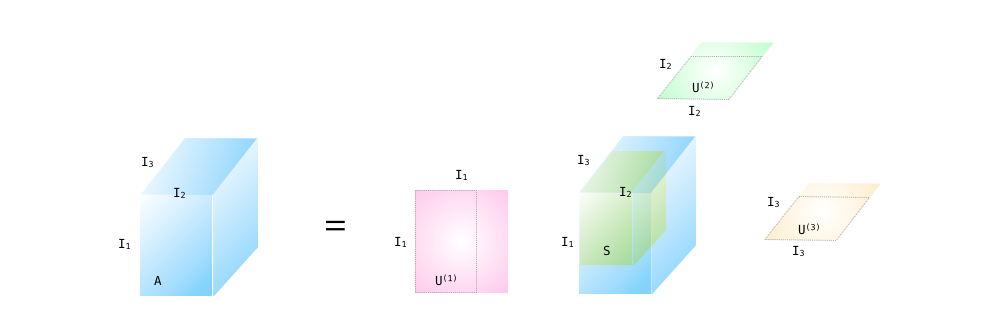
\includegraphics[width=1.00\textwidth]{figures/fig4311.png}
	\caption[The picture of the HOSVD for a rank-3 tensor.]{Picture of the HOSVD for a rank-3 tensor $A$. $U^{(1)}$,$U^{(2)}$ and $U^{(3)}$ are unitary matrices and $S$ (yellow cuboid) is a core tensor.}
	\label{fig4311}
\end{figure}

According to the theorem of HOSVD \cite{}, every \textit{complex} ($ I_1 \times I_2 \times \dots \times I_N$)-tensor $A$ could be decompose to a \textit{core tensor} $S$ and other $n$-mode unitary matrix $U^{(n)}$, where the maximum of $n$ must be smaller than $N$,
\begin{align}
	A = S \times U^{(1)} \times U^{(2)} \times \dots \times U^{(n)}
\end{align} 
As shown in Fig. \ref{fig4311}, a rank-3 tensor $A$ is decomposed to a core tensor $S$ (yellow cuboid) and three unitary matrices obtaining from three different modes.  The core tensor $S$ is a \textit{complex} ($ I_1 \times I_2 \times \dots \times I_N$)-tensor and have some significant properties, \begin{enumerate}
	\item Row-orthogonal: Two subtensors $S_{\alpha}^{(n)}$ and $S_{\beta}^{(n)}$ are orthogonal when $\alpha \neq \beta$. 
		\begin{align}		
			\left\langle S^{(n)}_{\alpha},S^{(n)}_{\beta} \right\rangle \quad \text{, if} \quad \alpha = \beta
		\end{align}		
		In other words, no matter the shape of $S$, each rows are orthogonal.
	\item Ordering: The Frobenius-norms $\text{ } \norm{S^{(n)}_{i}} $ is ordered from large to small.
		\begin{align}		
			\norm{S^{(n)}_1} \geq \norm{S^{(n)}_2} \geq \dots \geq \norm{S^{(n)}_{I_n}} \geq 0,
		\end{align}		
		for all possible values of $n$.
\end{enumerate}
\begin{figure}[ht]
	\centering
	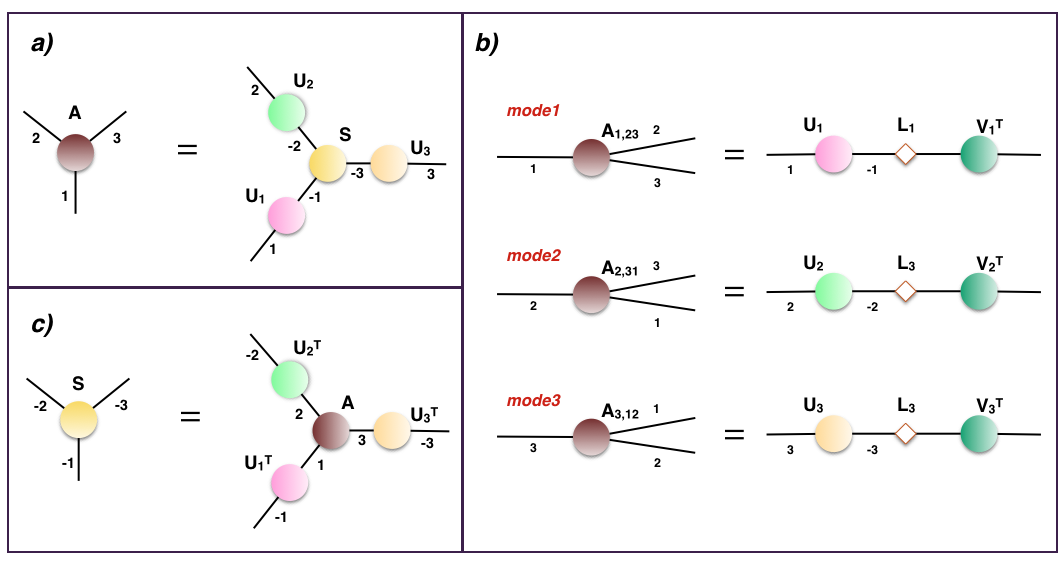
\includegraphics[width=0.90\textwidth]{figures/fig4312.png}
	\caption[The tensor-network representation of HOSVD]{(a) Decompose $A$ to a core tensor $S$ and $n$-mode unitary matrix $U^{(n)}$, (b) Obtain tensors $U^{(n)}$ from decomposing various modes of tensor $A$ by SVD, (c) Obtain the core tensor $S$ from contracting all transpose unitary tensors $U^{(n)T}$ }
	\label{fig4312}
\end{figure}
Now that we show the tensor-network representation for explaining more explicitly. If the target is to decompse a rank-3 $(N=3)$ tensor $A$ by 3 $(n=3)$ modes, see in Fig .\ref{fig4312}(a), we can implement is by the following steps, 
\begin{enumerate}
	\item	Reshaping the tensors to each modes and obtain $U^{(n)}$ by SVD , as shown in Fig. \ref{fig4312}(b).
	\item	Contract all $U^{(n)T}$ tensors for getting $S$ express more mathematically, 
		\begin{align}
			S = A \times U^{(1)T} \times U^{(2)T} \times \dots \times U^{(n)T}
		\end{align} 
		, see Fig. \ref{fig4312}(c).
\end{enumerate}
\subsection{Simple update for PESS}
In chapter.\ref{chapter:2ditebd}, we have introduced an efficient approximation, the "simple update", for determining the PEPS wave function. In principle, the wave function of PESS can be approached by the same way.
In PEPS structure, the ground-state wave function is approximated by iterated application of imaginary-time evolution operators $U(\tau) = e^{-\tau H}$ on an random PEPS state $\Ket{\Psi_t}$, where $\tau$ is a small constant, see Fig. \ref{fig312}. Base on the scheme, we can obtain the ground-state wave function of PESS by following steps,
\begin{enumerate}
	\item Split Hamiltonian $H$ to $H_{\alpha}$ and $H_{\beta}$ where $\alpha$ and $\beta$ are dependent on the geometry of the PESS structure.
	\item Obtain the evolution operator $U(\tau)$ by Trotter-Suzuki decomposition.
		\begin{align}
			e^{-\tau H} = e^{-\tau H_{\alpha}} e^{-\tau H_{\beta}} + O(\tau^{2}).
		\end{align}
	\item Absorb the environment bond vectors, which are considered as the entanglement between each simplex states, into projection tensors, and contract all projection tensors in the simplex state with the core tensor to obtain a cluster tensor.
	\item Apply the evolution operator $U$ to the cluster tensor for obtaining a new cluster tensor.
	\item Decompose the new cluster tensor by HOSVD.
	\item Truncate all the projection tensors and the core tensor.
	\item Absorb the inverse bond vectors for removing the entanglement on the projection tensors.
\end{enumerate}
In the following subsections, we applied various cases to explain it more explicitly.
\subsection{3-PESS and 5-PESS for infinite Kagome lattice}
\label{3-5pess}
\begin{figure}[ht]
	\centering
	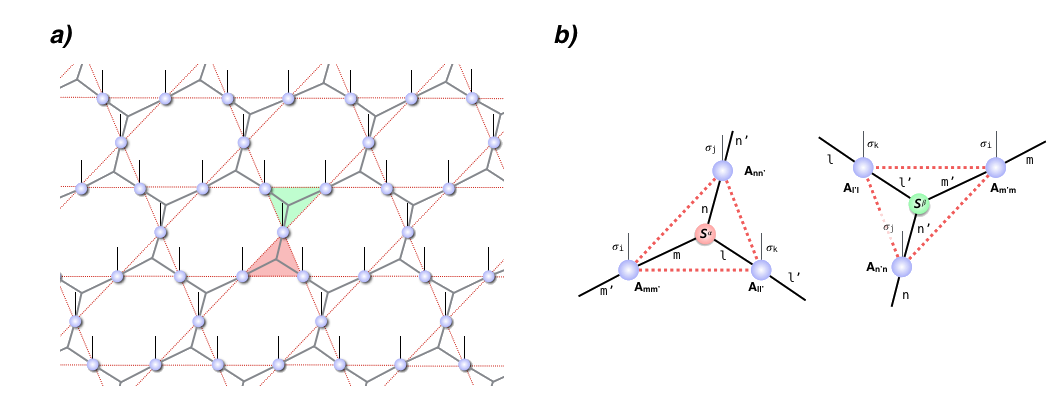
\includegraphics[width=1.00\textwidth]{figures/fig4321.png}
	\caption[The picture of the HOSVD for a rank-3 tensor.]{Picture of the HOSVD for a rank-3 tensor $A$. $U^{(1)}$,$U^{(2)}$ and $U^{(3)}$ are unitary matrices and $S$ (yellow cuboid) is a core tensor.}
	\label{fig4321}
\end{figure}
\begin{figure}[ht]
	\centering
	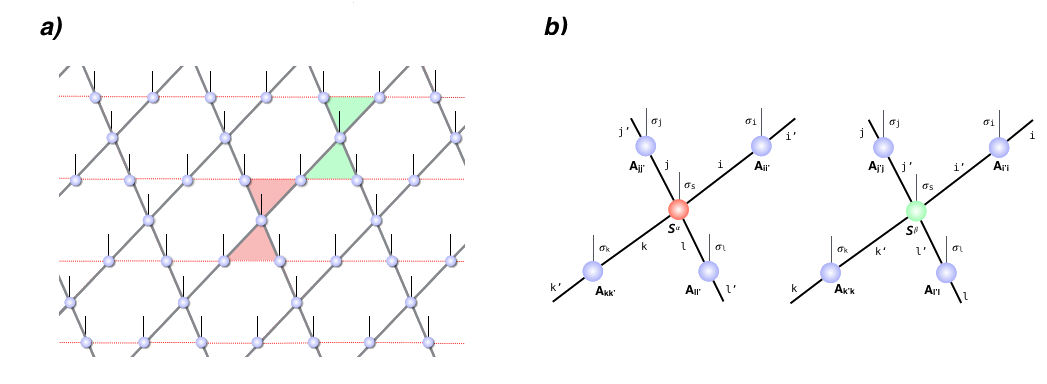
\includegraphics[width=1.00\textwidth]{figures/fig4322.png}
	\caption[The picture of the HOSVD for a rank-3 tensor.]{Picture of the HOSVD for a rank-3 tensor $A$. $U^{(1)}$,$U^{(2)}$ and $U^{(3)}$ are unitary matrices and $S$ (yellow cuboid) is a core tensor.}
	\label{fig4322}
\end{figure}

\begin{figure}[ht]
	\centering
	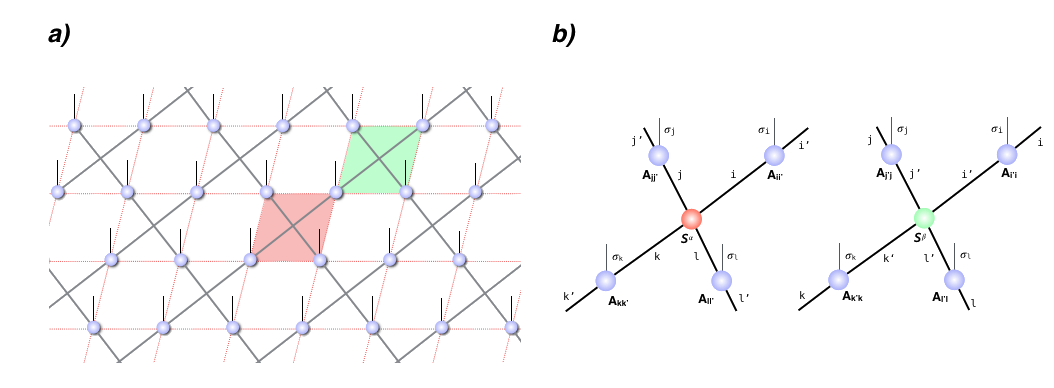
\includegraphics[width=1.00\textwidth]{figures/fig4323.png}
	\caption[The picture of the HOSVD for a rank-3 tensor.]{Picture of the HOSVD for a rank-3 tensor $A$. $U^{(1)}$,$U^{(2)}$ and $U^{(3)}$ are unitary matrices and $S$ (yellow cuboid) is a core tensor.}
	\label{fig4323}
\end{figure}
\begin{figure}[ht]
	\centering
	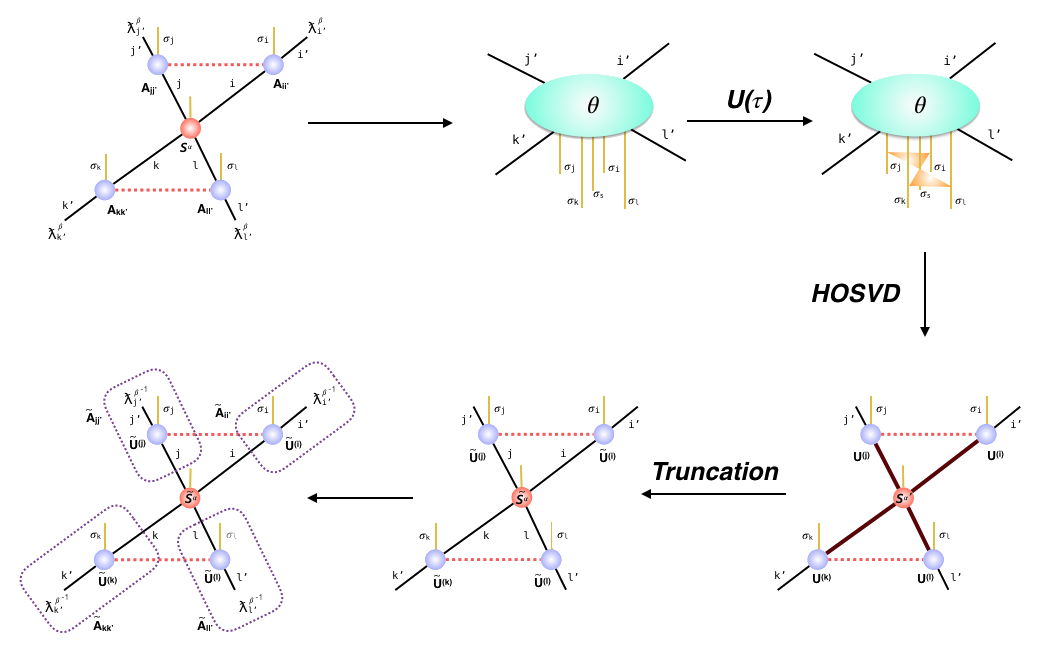
\includegraphics[width=1.00\textwidth]{figures/fig4324.png}
	\caption[The picture of the HOSVD for a rank-3 tensor.]{Picture of the HOSVD for a rank-3 tensor $A$. $U^{(1)}$,$U^{(2)}$ and $U^{(3)}$ are unitary matrices and $S$ (yellow cuboid) is a core tensor.}
	\label{fig4324}
\end{figure}

\subsection{4-PESS (Rank-3 local tensors) for Square lattice}
\label{4pess2b}
\begin{figure}[ht]
	\centering
	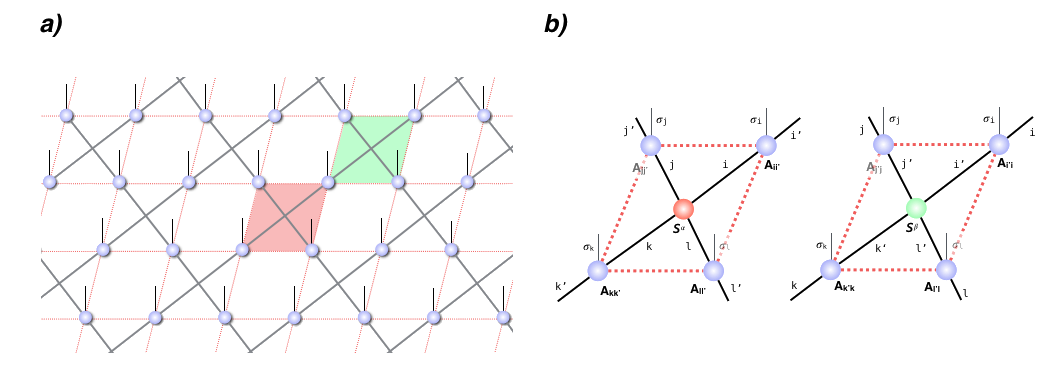
\includegraphics[width=1.00\textwidth]{figures/fig4325.png}
	\caption[The picture of the HOSVD for a rank-3 tensor.]{Picture of the HOSVD for a rank-3 tensor $A$. $U^{(1)}$,$U^{(2)}$ and $U^{(3)}$ are unitary matrices and $S$ (yellow cuboid) is a core tensor.}
	\label{fig4325}
\end{figure}
\begin{figure}[ht]
	\centering
	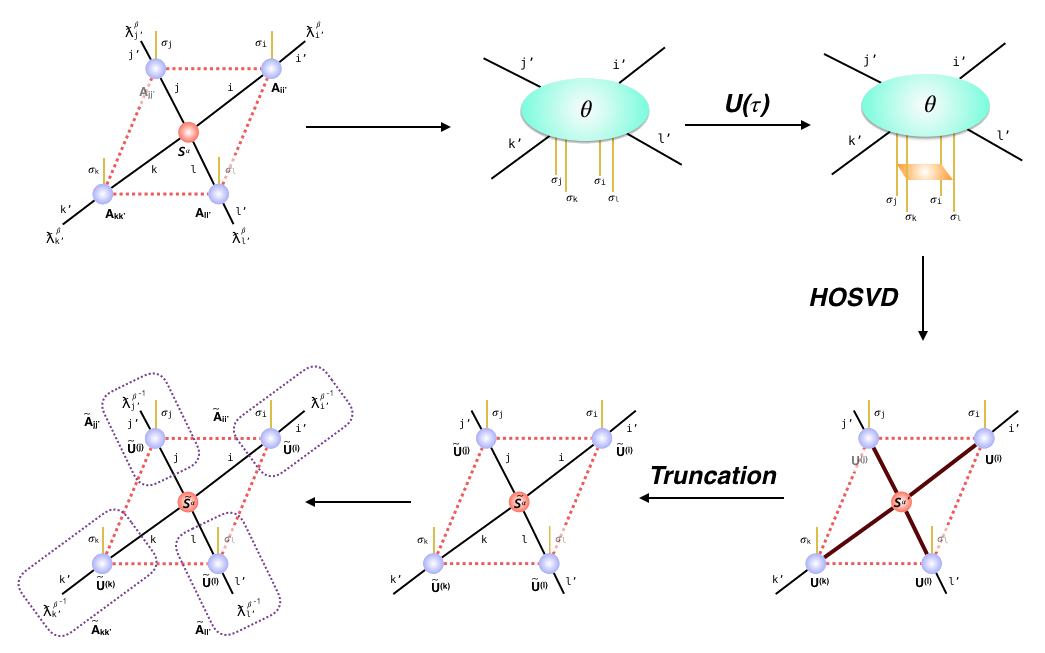
\includegraphics[width=1.00\textwidth]{figures/fig4326.png}
	\caption[The picture of the HOSVD for a rank-3 tensor.]{Picture of the HOSVD for a rank-3 tensor $A$. $U^{(1)}$,$U^{(2)}$ and $U^{(3)}$ are unitary matrices and $S$ (yellow cuboid) is a core tensor.}
	\label{fig4326}
\end{figure}
\subsection{4-PESS (Rank-5 local tensors)}
\label{4pess4b}

